\documentclass[11pt]{amsart}
\usepackage[all]{xy}
\usepackage[dvips]{graphicx}
\usepackage{amsfonts}
\usepackage{amssymb,latexsym,amsmath}
\usepackage{amsthm}
\usepackage{color}
\usepackage{empheq}
\usepackage{float}
\usepackage{hyperref}
\usepackage{listings}
\usepackage{mathrsfs}
\usepackage{slashed}
\usepackage{tikz}

\definecolor{dkgreen}{rgb}{0,0.6,0}
\definecolor{gray}{rgb}{0.5,0.5,0.5}
\definecolor{mauve}{rgb}{0.58,0,0.82}

\theoremstyle{definition}
\newtheorem{remark}{Remark}

\lstset{frame=tb,
    language=python,
    aboveskip=3mm,
    belowskip=3mm,
    showstringspaces=false,
    columns=flexible,
    basicstyle={\small\ttfamily},
    numbers=left,
    numberstyle=\tiny\color{gray},
    keywordstyle=\color{blue},
    commentstyle=\color{dkgreen},
    stringstyle=\color{mauve},
    breaklines=true,
    breakatwhitespace=true,
    tabsize=3
}

\textwidth = 420pt
\oddsidemargin = 18pt
\evensidemargin = 18pt

\begin{document}
\title{Cohort Revenue \& Retention Analysis: A Bayesian Approach}
\author{Juan Camilo Orduz}
\email{juanitorduz@gmail.com}
\urladdr{\href{https://juanitorduz.github.io/}{https://juanitorduz.github.io/}}
\address{Berlin, Germany}
\date{\today}

\begin{abstract}
    We present a Bayesian framework for jointly modeling cohort-level retention and revenue over time. We contribute a
    framework that couples these two business metrics through the number of active users. We model retention using Bayesian
    additive regression trees (BART) to capture non-linear patterns and seasonality, and couple this with a gamma-distributed
    revenue model where the estimated active user counts from the retention component inform the revenue predictions.
    This approach enables information sharing across cohorts, naturally incorporates seasonal effects, and
    provides well-calibrated uncertainty quantification through highest density intervals. The framework is flexible enough
    to incorporate additional covariates in both model components and can be implemented with alternative non-parametric
    approaches such as neural networks with stochastic variational inference. We demonstrate the approach using synthetic
    data designed to reflect realistic business scenarios, showing accurate out-of-sample predictions with appropriate
    uncertainty estimates. The framework's modular design facilitates extensions to hierarchical structures: we demonstrate
    a multi-market implementation that pools information across markets with varying data availability, enabling reliable
    forecasts even for markets with very limited cohort histories. Implementation code is provided in PyMC and NumPyro,
    making the method accessible for practical applications.
\end{abstract}

\maketitle

\addtocontents{toc}{\protect\setcounter{tocdepth}{1}}

\section{Introduction}

Understanding and predicting customer behavior directly impacts business profitability through improved retention strategies
and resource allocation. Among the metrics that define business success, retention and customer lifetime value
estimation stand at the forefront, serving as critical indicators of a company's ability to not only attract but maintain a
loyal customer base. These metrics transcend mere financial accounting—they represent the foundation upon which long-term
business strategies are built and refined. Seminal work by Fader and Hardie has established frameworks for both contractual
settings \cite{FaderHardie2007}, where subscription-based relationships predominate, and non-contractual settings
\cite{FaderHardie2005}, where customers may come and go without formal notification\footnote{Our definition of retention
    corresponds to what they call survival curve. See precise definitions below.}. Modern implementations of these CLV
models can now be found in Bayesian probabilistic programming frameworks such as PyMC (\cite{pymc2023}), where the
PyMC-Marketing library \cite{pymc_marketing} provides implementations of many standard buy-till-you-die (BTYD) models including
the BG/NBD, Pareto/NBD, and Gamma-Gamma models in a flexible, Bayesian framework. While these approaches have proven very valuable, they
often struggle to scale effectively. They can definitively be scaled with modern hardware and algorithms (for example,
stochastic variational inference, as described below). Nevertheless, this requires non-trivial work and effort.\\

For many decision-making processes, companies just need to understand behaviors at the cohort level—groups of customers
who joined during the same time period. In this paper we focus on this level of granularity. When shifting from individual
to cohort-level analysis, businesses typically face a methodological trilemma:

\begin{enumerate}
    \item \textbf{Complete pooling}: Aggregate all cohorts together and model retention and revenue as a collective whole,
          potentially obscuring important cohort-specific patterns.

    \item \textbf{No pooling}: Analyze each cohort in isolation, potentially overlooking valuable cross-cohort information
          and suffering from data sparsity for newer cohorts.

    \item \textbf{Partial pooling}: Model cohorts jointly with shared parameters, striking a balance between cohort-specific
          insights and statistical power.
\end{enumerate}

As detailed by \cite{FaderHardieNote2017}, each approach offers distinct advantages and limitations. However, a fundamental
challenge persists across these traditional methodologies: they typically lack the flexibility to efficiently incorporate
seasonality patterns and external regressors\footnote{Although, one can add regressors in some cases as described in
    \cite{FaderHardieNote2007} for the non-contractual case.}. This limitation becomes particularly problematic for businesses
with highly seasonal customer behavior—from retail operations affected by holiday shopping patterns to subscription services
influenced by annual promotional cycles. While some might argue that seasonality is secondary when estimating customer
lifetime value, the reality for many business models is that seasonal fluctuations significantly impact customer acquisition,
engagement, and retention decisions. Beyond the methodological challenges, businesses face practical hurdles in translating
retention and revenue models into actionable insights. Static models that fail to adapt to changing market dynamics or
consumer preferences quickly become outdated. Moreover, point estimates without associated uncertainty measures can lead to
misplaced confidence in business forecasts, potentially resulting in suboptimal resource allocation and strategic planning.

The economic value of improved retention and revenue forecasting extends across multiple business functions. More accurate
forecasts enable marketing teams to optimize customer acquisition spending by better estimating lifetime value, potentially
preventing over-investment in low-retention channels or under-investment in high-value segments. Financial planning becomes
more robust when forecasts include well-calibrated uncertainty estimates: rather than relying on single-point revenue
projections, organizations can quantify downside risks and plan accordingly. For subscription-based businesses in particular,
where customer retention directly determines revenue trajectory, forecast improvements of even 5-10\% in mean absolute error
can translate to substantially better resource allocation decisions. Moreover, probabilistic forecasts that capture
uncertainty—expressed through highest density intervals—enable risk-aware decision making, allowing organizations to tailor
strategies to their risk tolerance rather than treating uncertain outcomes as deterministic.

\subsection*{Why Cohort-Level Modeling?}

Before proceeding further, we address an important question: why focus on cohort-level rather than individual-level modeling?
While individual-level models can provide granular predictions for specific customers, cohort-level analysis offers several
strategic advantages that make it particularly well-suited for many business decision-making contexts.

First, cohort-level aggregation substantially reduces noise inherent in individual transaction data. Individual purchase
patterns are often highly variable and influenced by idiosyncratic factors that average out when aggregating to the cohort
level. This noise reduction leads to more stable parameter estimates and more reliable forecasts, particularly valuable for
strategic planning where robustness is paramount.

Second, cohort-level models align naturally with how many business decisions are actually made. Marketing strategies, budget
allocations, and resource planning typically target customer segments rather than individuals. Financial forecasting and
business planning operate at aggregate levels. A model that directly addresses these cohort-level questions provides more
immediately actionable insights than individual-level predictions that must subsequently be aggregated. This alignment
enhances accessibility for marketing stakeholders and strategic decision-makers who may not require customer-specific
granularity but need to understand temporal patterns and cohort dynamics.

Third, from a computational and practical perspective, cohort-level models scale more favorably than individual-level
approaches, particularly as customer bases grow into millions. While modern Bayesian methods can handle large individual-level
datasets, the computational requirements and implementation complexity increase substantially. Cohort-level modeling offers
an efficient path to actionable insights without sacrificing the flexibility to incorporate rich covariate information when
needed.

Importantly, the cohort-level focus does not preclude the incorporation of customer characteristics. As we demonstrate in our
framework, additional covariates—such as acquisition channel, geographic location, or customer segment—can be seamlessly
integrated into our model. To capture complex patterns in retention behavior without requiring explicit specification of
functional forms, we employ Bayesian Additive Regression Trees (BART) \cite{chipman2010bart}. BART is a flexible non-parametric
method that represents the unknown function as a sum of regression trees, allowing it to automatically learn non-linear
relationships and interactions between features. This flexibility is particularly valuable for cohort retention modeling, where
relationships between temporal features (cohort age, calendar time, seasonality) may be complex and difficult to specify
a priori. The non-parametric nature of BART allows it to scale effectively with many features, enabling the model to capture
heterogeneous effects across different customer types while maintaining the interpretability advantages of cohort-level
aggregation through tools like partial dependence plots. Thus, our approach strikes a balance: operating at the cohort level
for strategic clarity while retaining the flexibility to incorporate individual-level characteristics when they provide
additional explanatory power.

\subsection*{Related Work and Literature}

Our approach sits at the intersection of several research streams in customer analytics, survival analysis, and cohort
modeling. Understanding how our contribution relates to and extends existing methodologies is crucial for appreciating its
novelty and practical value.

\paragraph{Age-Period-Cohort Models.} The statistical literature on age-period-cohort (APC) modeling provides a rich
framework for understanding temporal patterns in grouped data. As comprehensively reviewed by \cite{fannon2018apc}, APC models
decompose outcomes into effects attributable to age (time since an event), period (calendar time effects), and cohort (group
membership defined by a common temporal characteristic). These models have found extensive application in demography,
epidemiology, and social sciences. However, traditional APC approaches face the well-known identification problem: age, period,
and cohort are linearly dependent (cohort + age = period), making their individual effects non-identifiable without additional
constraints. Moreover, standard APC models are typically specified for a single outcome variable, with additive decomposition
of age, period, and cohort effects. While APC models have been extended to multivariate settings in some contexts, the standard
framework and most applications focus on univariate outcomes. Our framework shares with APC models the recognition that outcomes
depend on age (time since cohort formation), period (calendar time), and cohort identity. However, rather than focusing on
decomposing and identifying separate age, period, and cohort effects—which requires imposing constraints or noting that only
non-linear components are identifiable—we use flexible non-parametric modeling with BART that captures the joint functional
relationship between these temporal dimensions without requiring explicit decomposition. Furthermore, we extend to joint
modeling of two related outcomes (retention and revenue) through a principled coupling mechanism.

\paragraph{Survival Analysis and Retention Modeling.} In the survival analysis literature, \cite{hubbard2021beta} recently
introduced Beta Survival Models that use non-parametric methods (including tree-based approaches) to model discrete-time
survival probabilities with a beta-logistic formulation. Their work demonstrates the value of flexible, non-parametric
approaches for capturing heterogeneous survival patterns and forecasting beyond observed horizons—capabilities that are
particularly relevant for retention modeling in business contexts. Our retention component shares the motivation of using
flexible non-parametric methods (BART in our case) to model time-to-churn patterns. However, we extend this foundation in
two critical directions. First, while \cite{hubbard2021beta} focus solely on survival/retention, we introduce a novel
coupling mechanism that connects retention to revenue through the number of active users, enabling joint forecasting of
both business-critical metrics. Second, our framework explicitly incorporates cohort structure and temporal effects in a
way that facilitates information sharing across cohorts—a feature absent from standard survival models but essential for
business applications where newer cohorts have limited historical data.

\paragraph{Customer Lifetime Value Models.} The customer lifetime value literature, pioneered by the work of Fader and
Hardie on buy-till-you-die (BTYD) models \cite{FaderHardie2005, FaderHardie2007}, provides powerful frameworks for
individual-level customer behavior modeling. These approaches, particularly the BG/NBD and Pareto/NBD models, have become
standard tools in marketing analytics. Modern Bayesian implementations in packages like PyMC-Marketing \cite{pymc_marketing}
have made these models more accessible and extended their capabilities. However, as previously noted, BTYD models operate
primarily at the individual level and can face scalability challenges. While \cite{FaderHardieNote2007} demonstrates that
covariates can be incorporated, and \cite{FaderHardieNote2017} discusses multi-cohort fitting strategies, these extensions
still work within the constraints of the original parametric model structures. Our approach complements this literature by
offering an alternative perspective: rather than aggregating individual-level predictions, we directly model cohort-level
patterns using flexible non-parametric methods that naturally capture complex interactions between temporal effects,
seasonality, and cohort characteristics.

\paragraph{Research Gaps and Our Contributions.} The existing literature reveals several gaps that our work addresses.
First, while age-period-cohort models provide a framework for temporal decomposition, they lack the flexibility to
capture non-linear patterns and are typically not designed for joint modeling of multiple related outcomes. Second, survival
analysis approaches focus on single outcomes (survival/retention) and do not provide mechanisms for connecting retention
to downstream business metrics like revenue. Third, traditional CLV models, while powerful for individual-level prediction,
can struggle with computational scalability and may not naturally incorporate rich temporal patterns like seasonality without
significant modeling effort. Our framework addresses these gaps through: (1) flexible non-parametric modeling via BART that
captures complex temporal patterns without requiring explicit functional form specification, (2) a novel coupling mechanism
that jointly models retention and revenue while preserving interpretability, (3) principled Bayesian uncertainty
quantification through posterior distributions rather than point estimates, and (4) efficient cohort-level aggregation that
balances statistical power with practical scalability. In the following sections, we formalize this framework and demonstrate
its effectiveness. \\

Having established the motivation and positioned our work within the broader literature, we now turn to describing the
modeling approach in detail. To get a visual intuition of the data we want to model, Figure \ref{fig:retention_matrix}
shows an example of a retention matrix. Here we encode the cohort retention as a function of time. Note that we exclude
the diagonal as it is uninformative (always containing ones). Observe that older cohorts have more data (obviously), so
we would like to use this information to improve the estimation of retention for younger cohorts. Hence, we do not want
to model each cohort independently but rather the {\em whole retention matrix} (we will do the same for the revenue
matrix and couple them together). \\

\begin{figure}
    \centering
    \includegraphics[width=\textwidth]{images/revenue_retention_17_0.png}
    \caption{Retention matrix example. The matrix visualizes customer retention rates across different cohorts (rows) and
        observation periods (columns). Each cell represents the proportion of customers from a specific acquisition
        cohort that remained active in a subsequent period. Colors indicate retention rates, with darker colors typically
        showing higher retention. This visualization allows for identifying cohort-specific patterns, seasonal effects,
        and retention decay over time. The diagonal is excluded as it always contains trivial values of 1 (100\%
        retention) for the cohort's first period.}
    \label{fig:retention_matrix}
\end{figure}

In addition, as we want to understand the monetary contribution of each cohort, we can consider the revenue matrix as shown
in Figure \ref{fig:revenue_matrix}. As in the retention case, we want to make sure we use all the information available to
improve the estimation of revenue for younger cohorts. Moreover, as we will discuss below, we will couple the retention and
revenue matrices through the number of active users, making the model structure very transparent for the business users
and stakeholders.

\begin{figure}
    \centering
    \includegraphics[width=\textwidth]{images/revenue_retention_23_0.png}
    \caption{Revenue per cohort. This heatmap visualizes the total revenue generated by each cohort (rows) across different
        time periods (columns). The color intensity corresponds to revenue magnitude, revealing a strong correlation
        with the number of active users (Figure \ref{fig:active_users}).}
    \label{fig:revenue_matrix}
\end{figure}

This approach offers several distinct advantages:

\begin{itemize}
    \item \textbf{Flexibility in relationship modeling}: By employing Bayesian additive regression trees (BART)
          \cite{quiroga2022bart}, our approach can capture complex non-linear relationships between cohorts, time periods,
          and behavioral metrics without requiring explicit specification of these relationships.

    \item \textbf{Integrated seasonality}: The model naturally incorporates seasonal patterns without requiring separate
          components or preprocessing steps.

    \item \textbf{Extensibility}: Additional covariates—from macroeconomic indicators to marketing campaign intensities—can
          be seamlessly integrated into the model.

    \item \textbf{Uncertainty quantification}: The Bayesian framework provides natural uncertainty estimates around all
          predictions, enabling risk-aware decision making.

    \item \textbf{Information sharing across cohorts}: Newer cohorts with limited historical data benefit from patterns
          learned from more established cohorts.
\end{itemize}

An important strength of this modular framework is its extensibility to more complex structures. To illustrate, we present
a hierarchical extension that models multiple markets simultaneously, pooling information across them. This is particularly
valuable when some markets have limited data: by sharing information through hierarchical priors, we can generate reliable
forecasts for young markets that would be impossible to model in isolation. The hierarchical implementation, detailed in
Section 6, demonstrates how naturally the framework accommodates such extensions without fundamental redesign.

Specifically, we use Bayesian additive regression trees to model the retention component, capturing the probability that a
customer from a given cohort remains active in subsequent periods. We couple this with a linear model for the revenue
component, predicting how much revenue active customers will generate. This dual approach balances the flexibility needed to
capture complex retention patterns with the interpretability desired for revenue forecasting. Next we describe the main
ingredients of our model: the features and the model specification. We will delve into the details in the next sections.

\subsection*{Features}

Typical purchase databases contain transactional history at user level. We want an approach general enough to benefit
from the most common features instead of heavy feature engineering. Going back to Figure \ref{fig:retention_matrix}, it
is natural to consider the following features to model the retention and revenue matrices:

\begin{itemize}
    \item {\bf Cohort age}: Age of the cohort in months, representing the time since the cohort was formed.
    \item {\bf Age}: Age of the cohort with respect to the observation time.
          This feature serves as a numerical encoder for the cohort's position in time.
    \item {\bf Month}: Month of the observation time (period), capturing seasonality effects.
\end{itemize}

For example, if our observation month is {\em 2022-11} and we consider the cohort {\em 2022-09}, the age of this cohort
is $2$ months, as the age is always calculated relative to the observation period. This cohort was observed during two
periods: {\em 2022-10} and {\em 2022-11} with cohort ages $1$ and $2$ respectively. \\

All these features are available for out-of-sample predictions, ensuring model applicability for forecasting.
In practice, we can add additional covariates to the model. The only requirement for out-of-sample predictions is that
these covariates must be available for future observation periods.

\subsection*{Model Specification}

The main idea behind the specification is to model each revenue and retention matrices, using the features above, and
couple them together. Specifically, we have:

\begin{itemize}
    \item {\bf Retention Component}: We model the number of active users $N_{\text{active}}$ in each cohort as a binomial random
          variable $\text{Binomial}(N_{\text{total}}, p)$, where the parameter $p$ represents the retention probability
          (see Figure \ref{fig:active_users}, from a synthetic example described below). We model the latent variable $p$
          using a BART model with features cohort age, age, and month. This flexible approach allows the model to
          capture non-linear relationships and interactions between features.

    \item {\bf Revenue Component}: We model the revenue matrix (see Figure \ref{fig:revenue_matrix}) through a gamma random variable
          $\text{Gamma}(N_{\text{active}}, \lambda)$, as we want to ensure non-negative values. We model the rate parameter
          $\lambda$ through a linear model with features cohort age, age, and a multiplicative interaction term (using a
          $\log$ link function). We do not explicitly add a seasonality component to this part of the model, as we typically
          observe that most seasonality effects are already captured by the retention component. However, seasonal features
          could be added if needed (plus additional features and different parametrizations, for example multiplicative
          effects).

    \item {\bf Coupling}: The retention and revenue coupling is a key feature of this work. We couple the two components
          through the number of active users, extending decomposition ideas similar to those in the Gamma-Gamma model from the
          CLV literature, which separates transaction frequency from monetary value. Here is the full model specification:

          \begin{align*}
              \text{Revenue}    & \sim \text{Gamma}(N_{\text{active}}, \lambda)                                             \\
              \log(\lambda) = ( & \text{intercept}                                                                          \\
                                & + \beta_{\text{cohort age}} \times \text{cohort age}                                      \\
                                & + \beta_{\text{age}} \times \text{age}                                                    \\
                                & + \beta_{\text{cohort age} \times \text{age}} \times \text{cohort age} \times \text{age}) \\
              N_{\text{active}} & \sim \text{Binomial}(N_{\text{total}}, p)                                                 \\
              \textrm{logit}(p) & = \text{BART}(\text{cohort age}, \text{age}, \text{month})
          \end{align*}

\end{itemize}

\begin{figure}
    \centering
    \includegraphics[width=\textwidth]{images/revenue_retention_21_0.png}
    \caption{Number of active users across cohorts. This heatmap displays the absolute count of active users for each
        cohort (rows) across observation periods (columns).}
    \label{fig:active_users}
\end{figure}

\begin{figure}
    \centering
    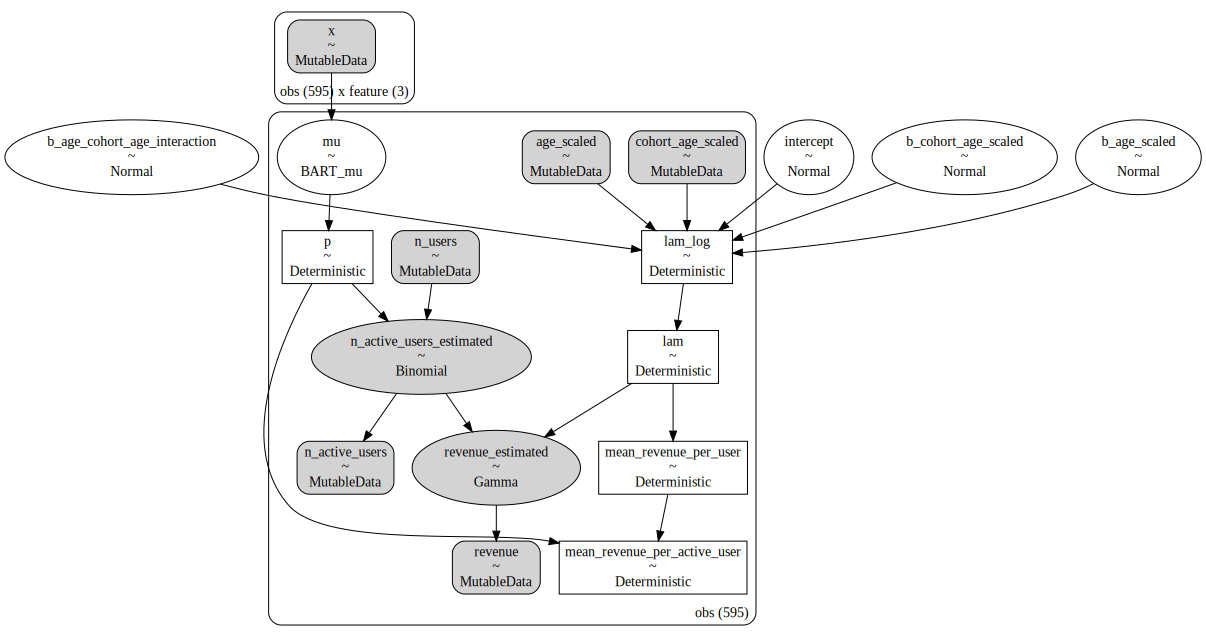
\includegraphics[width=\textwidth]{images/revenue_retention_33_0.png}
    \caption{Cohort-revenue-retention model structure. This diagram illustrates the coupling mechanism that connects
        the two components of our framework. On the left, the retention component models the number of active users
        $N_{\text{active}}$ as a binomial random variable, where the retention probability $p$ is modeled using BART with
        features including cohort age, age (cohort identifier), and month (seasonality). On the right, the revenue component
        models total revenue as a gamma-distributed random variable, with the shape parameter directly determined by
        $N_{\text{active}}$ from the retention model. This coupling through active users provides a natural connection:
        changes in retention patterns automatically propagate to revenue predictions, ensuring consistency between the two
        metrics while allowing each component to use appropriate distributional assumptions and feature sets.}
    \label{fig:revenue_retention_model}
\end{figure}

Figure \ref{fig:revenue_retention_model} illustrates the complete model structure. Our goal is to simultaneously estimate
the BART parameters and the beta coefficients (including the intercept) of the linear component. We want to do this to
understand the contribution of each feature to the retention and revenue over time. Additionally, to operationalize the
model, we will use the retention and revenue matrices to make out-of-sample predictions. This can be extremely important
for scenario and business planning. A typical application is to use this model to generate {\em counterfactuals} for
global interventions where we expect different cohorts to react differently. \\

In the rest of the paper, we delve into the details of the model specification and diagnostics. Moreover, we describe
how to generate out-of-sample predictions for both the retention and revenue matrices. \\

To make the approach more tangible,
we present a synthetic dataset in the next section. This should help the reader to better understand the data and the approach.

\section{Synthetic Data}

Having established the theoretical foundations and positioning of our approach, we now turn to a concrete demonstration using
synthetic data. While our framework has been successfully applied to real business datasets, we present results using synthetic
data for reproducibility and to avoid proprietary information concerns. The synthetic dataset is designed to reflect realistic
business scenarios, incorporating the types of temporal patterns and cohort dynamics commonly observed in subscription-based
and retention-focused business models.

The synthetic dataset is available as a CSV file from \cite{orduz_revenue_retention}, and the code to generate this dataset
deterministically is publicly available in \cite{orduz_revenue_retention_data_code}. This ensures full reproducibility of
our results and allows researchers to explore model behavior under controlled conditions.

\subsection*{Exploratory Data Analysis}

Before fitting our model, we conduct exploratory data analysis to understand the key patterns in the data. This analysis
both motivates our modeling choices and provides a baseline for evaluating model performance. Figure \ref{fig:retention_matrix}
displays the retention matrix per cohort and period. Two key observations stand out:

\begin{enumerate}
    \item The retention exhibits a clear seasonal pattern with respect to the period, being higher in the last months of the
          year and lower in the middle of the year. This seasonality pattern is more evident in Figure
          \ref{fig:retention_seasonal}.
    \item Retention appears to increase as the cohort age decreases. This trend is apparent when comparing retention values
          for periods in November across different cohort ages.
\end{enumerate}

\begin{figure}
    \centering
    \includegraphics[width=\textwidth]{images/revenue_retention_19_0.png}
    \caption{Retention as a function of the period, demonstrating the yearly seasonality pattern in retention values.}
    \label{fig:retention_seasonal}
\end{figure}

It's important to remember that retention is a ratio, making cohort size an important factor. For instance, a retention rate
of 0.4 could represent either $4/10$ or $4\times 10^{5} / 10^{6}$. The former case carries considerably more uncertainty in
its estimation. This insight motivates us to examine the number of active users, as shown in Figure \ref{fig:active_users}.
We observe that more recent cohorts have significantly more active users, a pattern we want our model to account for. \\

Next, we examine revenue patterns. Figure \ref{fig:revenue_matrix} presents revenue by cohort, showing a strong correlation with the
number of active users. This suggests that revenue per user remains relatively stable over time. To verify this, we compute
revenue per user as a function of age and period (Figure \ref{fig:revenue_per_user}) as well as revenue per {\em active} user
(Figure \ref{fig:revenue_per_active_user}). The key difference between these metrics is that revenue per user divides by
total cohort size, while revenue per active user divides by the number of active users in the given period. All in all,
we observe the following for the revenue data\footnote{These types of patterns are actually common in real applications. This synthetic
    dataset is motivated by real applications where the model was proven to be very effective}:

\begin{itemize}
    \item Revenue per user exhibits a clear seasonality pattern, consistent with the seasonal pattern observed in retention.
    \item Revenue per active user does not show the same seasonality pattern since seasonal effects are already captured in
          the denominator (active users). Additionally, revenue per active user appears to decrease as cohort age increases,
          suggesting that older cohorts generate less revenue per active customer. \\
\end{itemize}

These exploratory findings inform our modeling strategy. The strong seasonality in retention motivates the inclusion of
month (period) as a feature in the BART component. The heterogeneity across cohort ages suggests that flexible non-parametric
modeling will be valuable for capturing these varying patterns. The relationship between revenue and active users justifies
our coupling mechanism, while the patterns in revenue per active user guide the parametric specification of the revenue
component. With this exploratory understanding established, we now proceed to formalizing and fitting our model.

\begin{figure}
    \centering
    \includegraphics[width=\textwidth]{images/revenue_retention_27_0.png}
    \caption{Revenue per user across cohorts. This visualization normalizes the total revenue by the original cohort size,
        showing the average revenue generated per initially acquired user.}
    \label{fig:revenue_per_user}
\end{figure}

\begin{figure}
    \centering
    \includegraphics[width=\textwidth]{images/revenue_retention_25_0.png}
    \caption{Revenue per active user across cohorts. This metric divides total revenue by the number of active users in each
        period, isolating spending patterns from retention effects.}
    \label{fig:revenue_per_active_user}
\end{figure}

\section{Model Structure and Diagnostics}

\subsection{Model Specification}

Let's expand on the model structure outlined in the introduction. The core concept is to model the number of active users
as a binomial random variable $N_{\text{active}} \sim \text{Binomial}(N_{\text{total}}, p)$, where $p$ represents the retention
probability. We use Bayesian additive regression trees (BART) to model this latent variable $p$ using cohort age, age, and
month (period) as features.

\begin{align*}
    N_{\text{active}} & \sim \text{Binomial}(N_{\text{total}}, p)                  \\
    \textrm{logit}(p) & = \text{BART}(\text{cohort age}, \text{age}, \text{month})
\end{align*}

It is important to clarify the role of $N_{\text{active}}$ in the model specification versus estimation. In the model
formulation above, $N_{\text{active}}$ is formally treated as a random variable following a binomial distribution. However,
in practical applications with observed cohort data, we directly observe retention rates (the proportion of customers who
remain active) or equivalently, the realized counts $N_{\text{active}}$. During inference, the observed retention data
informs the estimation of $p$ through the BART model, which captures how retention probability varies across cohorts, time
periods, and months. This formulation allows us to propagate uncertainty from the retention probability estimates through
to revenue predictions via the coupling mechanism described below.

\paragraph{BART Prior Specification.} BART models the unknown retention function as a sum of many regression trees, where
each tree contributes a small part to the overall prediction \cite{chipman2010bart}. The key advantage is that this ensemble
automatically learns complex non-linear patterns and interactions without requiring the analyst to specify functional forms.
The prior specification encourages sparse, shallow trees that collectively capture the data structure while avoiding overfitting.

We implement BART using the PyMC framework via \cite{quiroga2022bart}, which handles the technical details of tree structure
priors and parameter estimation. The main tuning parameter is the number of trees $m$. We use default prior settings from
\cite{chipman2010bart} which have proven robust across diverse applications: these priors favor shallow trees and regularize
individual tree contributions so that the ensemble learns smooth functions through additive combinations. For our retention
modeling, we typically start with $m = 20$ trees and increase incrementally (e.g., to 50 or 100) while monitoring posterior
predictive fit. BART is relatively insensitive to this choice for sufficiently large $m$, but smaller values offer
computational efficiency and maintain interpretability through tools like partial dependence plots.

Readers interested in the mathematical details of BART priors—including tree topology priors, splitting rule distributions,
and leaf parameter specifications—are referred to the comprehensive treatment in \cite{chipman2010bart} and the implementation
details in \cite{quiroga2022bart}.

\begin{remark}
    A key advantage of the BART model is its flexibility in incorporating additional covariates. In real business
    applications, we have successfully added customer segmentation features (such as acquisition media channels from
    attribution models). This provides valuable insights into media channel return-on-investment (ROI), allowing businesses
    to consider not just acquisition costs but also estimated customer lifetime value through this combined model.
\end{remark}

\begin{remark}
    While one could start with a simpler model, such as a linear model as described in \cite{orduz_revenue_retention},
    our experience with real datasets shows that such simpler approaches often fail to adequately capture the complex
    patterns in the data.
\end{remark}

\paragraph{Computational Details and Inference.} Inference for BART models is performed using Markov Chain Monte Carlo (MCMC)
methods, specifically the Particle Gibbs sampler implemented in \cite{quiroga2022bart}. This algorithm iteratively updates
tree structures through propose-accept-reject steps and updates leaf parameters through Gibbs sampling conditional on the
tree structures. The MCMC sampler requires specification of the number of chains, number of draws, and warm-up (burn-in)
period. We use multiple chains (typically 4) to assess convergence through standard diagnostics. For the synthetic data
analysis presented in this paper, we run 2000 draws with 1000 warm-up iterations per chain, which proves sufficient for
convergence. Larger datasets or more complex models may require more iterations.

Convergence diagnostics play a crucial role in ensuring reliable inference. We monitor the $\hat{R}$ statistic (Gelman-Rubin
diagnostic) for all parameters, requiring $\hat{R} < 1.01$ for convergence. We also visually inspect trace plots for the
linear model parameters to ensure proper mixing and stationarity. The BART component's stochastic nature (sampling tree
structures) means individual tree parameters are not directly interpretable, but we can assess overall model convergence
through the posterior predictive distribution and by monitoring whether different chains produce similar predictions. We
verify that the model produces no divergent transitions, which would indicate problematic posterior geometry. All diagnostics
are implemented using the ArviZ library for exploratory analysis of Bayesian models.

For the revenue component, we employ a gamma random variable $\text{Gamma}(N_{\text{active}}, \lambda)$ (inspired by
\cite{stucchio2015bayesian}). The gamma distribution is a natural choice for modeling revenue as it ensures non-negativity
and provides flexibility in capturing different revenue distributions through its shape and rate parameters. The mean of
this gamma distribution is $N_{\text{active}} / \lambda$, allowing us to interpret $1 / \lambda$ as the {\em average
revenue per active user}. By using $N_{\text{active}}$ as the shape parameter, we ensure that cohorts with more active
users have lower relative variance (coefficient of variation $1/\sqrt{N_{\text{active}}}$), which aligns with the intuition
that aggregated revenue from larger cohorts should be more stable. This parametrization also creates a direct connection
between the retention and revenue components: cohorts with higher retention (larger $N_{\text{active}}$) contribute both
higher expected revenue and more concentrated revenue distributions. We model $\log(\lambda)$ using a linear function of
cohort age, age, and their interaction. As a preprocessing step, we standardize these features for the linear model component
(we keep the same notation for the variables for simplicity). This allows us to specify priors for the regression coefficients
in terms of the effect of a one-standard-deviation change in the predictor, enabling effective regularization through standard
normal priors for the coefficients (see \cite{orduz_retention_bart}).

\begin{align*}
    \text{Revenue}    & \sim \text{Gamma}(N_{\text{active}}, \lambda)                                             \\
    \log(\lambda) = ( & \text{intercept}                                                                          \\
                      & + \beta_{\text{cohort age}} \times \text{cohort age}                                      \\
                      & + \beta_{\text{age}} \times \text{age}                                                    \\
                      & + \beta_{\text{cohort age} \times \text{age}} \times \text{cohort age} \times \text{age})
\end{align*}

A key insight from both this synthetic dataset and many real-world applications is that we typically don't need to explicitly
model seasonality in the revenue component, as seasonal patterns are already captured by the retention component.

\begin{remark}
    The {\em age} feature characterizes each cohort's temporal position. While we could replace this numerical encoding with
    a one-hot encoding of cohorts and add hierarchical structure to pool information across cohorts, the numerical encoding
    is more parsimonious under the assumption that temporally proximate cohorts behave more similarly than distant ones.
\end{remark}

In summary, our cohort-revenue-retention model is specified as:

\begin{align*}
    \text{Revenue}                              & \sim \text{Gamma}(N_{\text{active}}, \lambda)                                             \\
    \log(\lambda) = (                           & \text{intercept}                                                                          \\
                                                & + \beta_{\text{cohort age}} \times \text{cohort age}                                      \\
                                                & + \beta_{\text{age}} \times \text{age}                                                    \\
                                                & + \beta_{\text{cohort age} \times \text{age}} \times \text{cohort age} \times \text{age}) \\
    N_{\text{active}}                           & \sim \text{Binomial}(N_{\text{total}}, p)                                                 \\
    \textrm{logit}(p)                           & = \text{BART}(\text{cohort age}, \text{age}, \text{month})                                \\
    \text{intercept}                            & \sim \text{Normal}(0, 1)                                                                  \\
    \beta_{\text{cohort age}}                   & \sim \text{Normal}(0, 1)                                                                  \\
    \beta_{\text{age}}                          & \sim \text{Normal}(0, 1)                                                                  \\
    \beta_{\text{cohort age} \times \text{age}} & \sim \text{Normal}(0, 1)
\end{align*}

\subsection{Diagnostics}

With the model fully specified, we implement and fit it using PyMC \cite{pymc2023}, leveraging the BART implementation
from \cite{quiroga2022bart}. Complete implementation details and code are available in \cite{orduz_revenue_retention}. After
fitting the model using MCMC with the computational settings described above, we conduct thorough diagnostics to ensure
reliable inference.

Figure \ref{fig:posterior_predictive} presents a critical diagnostic: the posterior predictive distribution for both model
components. These plots compare the distribution of observed values against the distribution of values simulated from the
fitted model's posterior predictive distribution. Close agreement between these distributions indicates that the model
successfully captures the data-generating process. For both retention and revenue components, we observe excellent agreement,
with the simulated distributions (orange) closely matching the observed distributions (black). This suggests the model
provides an adequate fit to the data.

Beyond the posterior predictive check, we examine convergence diagnostics for the model parameters. Figure \ref{fig:trace}
displays trace plots for the linear model parameters (intercept and regression coefficients). These plots show the evolution
of parameter values across MCMC iterations for each chain. Good mixing—evidenced by chains that explore the parameter space
efficiently without getting stuck—is essential for reliable inference. We observe healthy mixing for all parameters, with no
divergences or convergence warnings. All $\hat{R}$ statistics are below 1.01, confirming convergence. These diagnostics give
us confidence that the MCMC sampling has successfully explored the posterior distribution and that our parameter estimates
are reliable.

\begin{figure}
    \centering
    \includegraphics[width=\textwidth]{images/revenue_retention_37_0.png}
    \caption{Posterior predictive distribution of the retention (left) and revenue (right) components, showing good fit to
        the observed data. These cumulative density plots compare the distributions of observed values (black) with simulated
        values from the posterior predictive distribution (orange), providing a visual assessment of model fit.}
    \label{fig:posterior_predictive}
\end{figure}

\begin{figure}
    \centering
    \includegraphics[width=\textwidth]{images/revenue_retention_41_0.png}
    \caption{Trace plots for the linear model parameters, showing good mixing and convergence of the MCMC chains.}
    \label{fig:trace}
\end{figure}

\subsection{Variable Importance}

A key advantage of using BART over more opaque machine learning methods is the availability of tools for understanding which
features drive predictions and how they influence outcomes. The BART implementation in \cite{quiroga2022bart} provides
interpretability tools that allow us to peer inside the model and extract actionable insights about retention drivers.

Figure \ref{fig:ice_plot} presents PDP (Partial Dependence Plot) and ICE (Individual Conditional Expectation) plots for the
retention component. These visualization techniques reveal how the model's predictions change as each feature varies
while holding all other features constant. Each line represents a different observation from the dataset, showing how the
predicted retention probability would change for that observation if we modified only the feature of interest. The PDP
plot is the average of the ICE plots (solid line). These plots allow us to understand how the retention probability varies
for different values of the features and reveals potential non-linear relationships or interaction effects that might not
be apparent in aggregate statistics. \\

\begin{figure}
    \centering
    \includegraphics[width=\textwidth]{images/retention_bart_32_1.png}
    \caption{Partial Dependence Plot (PDP, solid lines) and Individual Conditional Expectation (ICE, thin dashed lines) plots
        for the retention component. These plots visualize how the predicted retention probability changes as each feature
        varies while holding others constant. The left panel shows the effect of cohort age: retention decreases as cohorts
        mature, with relatively consistent patterns across observations. The middle panel displays the age (cohort identifier)
        effect: more recent cohorts tend to have higher retention. The right panel reveals strong seasonality: retention
        peaks in months 11-12 (November-December) and dips in mid-year months. The close alignment between individual ICE
        plots and the average PDP suggests relatively consistent feature effects across different observations, indicating
        limited interaction effects. These plots demonstrate one of BART's key advantages: interpretable visualization of
        learned patterns without requiring pre-specification of functional forms.}
    \label{fig:ice_plot}
\end{figure}

In this specific example, we can extract the following insights:

\begin{itemize}
    \item The ICE plots show how the retention rate decreases with both cohort age and age. This is not surprising as we saw in the EDA.
    \item We see that the ICE plots have a similar trend to the PDP plots. This hints that the interaction effects are
          not so important in this case. This is also something we saw in the linear model where the interaction coefficient
          was relatively small (see \cite{orduz_retention}).
    \item We clearly see the seasonality component of the PDP / ICE plots resemble the regression coefficients in the linear
          model from \cite{orduz_retention}. This is simply representing the strong seasonal component of the data.
\end{itemize}

In addition, we can extract a relative importance for the different features using the contribution to the in-sample $R^2$,
as shown in Figure \ref{fig:variable_importance}.

\begin{figure}
    \centering
    \includegraphics[width=\textwidth]{images/retention_bart_32_0.png}
    \caption{Variable importance for the retention component, quantified by each feature's contribution to in-sample $R^2$.
        This metric captures how much predictive power each feature adds to the model. Month (period) emerges as the most
        important feature, reflecting the strong seasonality observed in the exploratory analysis. Cohort age is also highly
        important, capturing the decay in retention as cohorts mature. The age (cohort identifier) has lower but non-negligible
        importance, suggesting some differences between cohorts beyond what is captured by cohort age and seasonality. These
        importance scores help prioritize data collection efforts and guide model simplification if needed, though all three
        features clearly contribute meaningfully to retention prediction.}
    \label{fig:variable_importance}
\end{figure}

These types of plots are very valuable to understand the {\em drivers} of the retention component.

\section{Predictions}

Having established that our model fits the data well and that MCMC sampling has converged, we now examine the model's
predictive performance. This section evaluates predictions in two contexts: in-sample predictions that assess how well the
model captures observed patterns, and out-of-sample predictions that test the model's ability to forecast future retention
and revenue for periods beyond the training data. The distinction is crucial: in-sample fit demonstrates that the model
adequately represents the data-generating process, while out-of-sample performance reveals whether the model generalizes to
new data—the ultimate test for any predictive framework intended for business forecasting.

\subsection{In-Sample Predictions}

We first evaluate the model's in-sample performance by comparing the posterior predictive mean against the observed values.
Figure \ref{fig:in_sample_mean} shows the comparison for both retention and revenue components, with points closer to the
diagonal line indicating better fit. Beyond point estimates, we can visualize the full posterior predictive distribution
to assess model uncertainty. Figure \ref{fig:in_sample_retention} shows the posterior predictive distribution of retention
for selected cohorts, with $94\%$ HDI (Highest Density Interval). Note how the intervals are narrower for more recent
cohorts with more data, reflecting greater certainty in these predictions. Overall, the predictions effectively capture the
observed retention patterns, including seasonality. For the revenue component, Figure \ref{fig:in_sample_revenue} shows
the posterior predictive distribution compared to actual revenue values. The model successfully captures the revenue
variability across different cohorts and time periods. We can use the whole posterior distribution to make custom visualizations
of quantities of interests like the revenue per active user, as shown in Figure \ref{fig:additional_predictions}.

\begin{figure}
    \centering
    \begin{tabular}{cc}
        \includegraphics[width=0.5 \textwidth]{images/revenue_retention_45_0.png} &
        \includegraphics[width=0.5 \textwidth]{images/revenue_retention_47_0.png}
    \end{tabular}
    \caption{Retention (left) and revenue (right) in-sample posterior predictive mean values plotted against the actual
        observations. These scatter plots provide a quantitative assessment of model fit by comparing predicted
        versus observed values, with points closer to the diagonal line indicating better predictions.}
    \label{fig:in_sample_mean}
\end{figure}

\begin{figure}
    \centering
    \includegraphics[width=\textwidth]{images/revenue_retention_51_0.png}
    \caption{Retention in-sample posterior predictive distribution for selected cohorts, showing $94\%$ HDI (blue shaded areas)
        and observed retention values (blue points). This visualization displays the model's predictive performance for
        retention across time for different cohorts, with uncertainty quantified through highest density intervals.
        The narrower intervals for more recent cohorts (bottom panels) reflect greater certainty due to more available
        data, while the consistent capture of observed values within the intervals indicates well-calibrated uncertainty
        estimates. The plots also reveal the model's ability to adapt to cohort-specific patterns and seasonal
        fluctuations, demonstrating its flexibility in capturing complex temporal dynamics.}
    \label{fig:in_sample_retention}
\end{figure}

\begin{figure}
    \centering
    \includegraphics[width=\textwidth]{images/revenue_retention_53_0.png}
    \caption{Revenue in-sample posterior predictive distribution for selected cohorts, showing $94\%$ HDI (blue shaded areas)
        and observed revenue values (blue points). These plots illustrate the model's revenue predictions and associated
        uncertainty across time for different cohorts. The successful capture of observed values within the HDI bands
        demonstrates the model's ability to accurately represent not just central tendencies but also the inherent
        variability in revenue. The visualization highlights how our coupled modeling approach effectively propagates
        uncertainty from the retention component to revenue estimates, providing business stakeholders with realistic
        confidence intervals for financial planning and analysis.}
    \label{fig:in_sample_revenue}
\end{figure}

\begin{figure}
    \includegraphics[width=\textwidth]{images/revenue_retention_56_0.png}
    \caption{Additional view of posterior predictions across cohorts, illustrating the model's ability to capture
        cohort-specific patterns. This panel view organizes predictions by cohort (columns) and shows how the model
        adapts to the unique characteristics of each customer group.}
    \label{fig:additional_predictions}
\end{figure}

\subsection{Out-of-Sample Predictions}

The true test of any predictive model is its performance on unseen data. We evaluate our model's forecasting capabilities
using a holdout set consisting of data after {\em 2022-11}, which was not used during model training. Figures
\ref{fig:out_sample_retention} and \ref{fig:out_sample_revenue} show the out-of-sample predictions for retention and
revenue, respectively. The vertical dashed lines indicate the train/test split point. Several key observations emerge:

\begin{enumerate}
    \item The model successfully predicts both retention and revenue patterns for future periods, with most actual
          observations falling within the $94\%$ HDI.

    \item The model effectively captures the seasonal patterns in retention, correctly predicting the expected peaks and
          troughs in future months based on historical patterns.

    \item For newer cohorts with limited training data (e.g., the {\em 2022-07} cohort with only 4 data points in
          training), the model still produces reasonable predictions by leveraging information learned from older cohorts.
          This demonstrates effective transfer of knowledge across cohorts.

    \item The $94\%$ HDI appropriately widens for more distant future predictions, reflecting increasing uncertainty as we
          forecast further ahead. \\
\end{enumerate}

\begin{figure}
    \centering
    \includegraphics[width=\textwidth]{images/revenue_retention_66_0.png}
    \caption{Retention out-of-sample posterior predictive distribution for (random) selected cohorts.}
    \label{fig:out_sample_retention}
\end{figure}

\begin{figure}
    \centering
    \includegraphics[width=\textwidth]{images/revenue_retention_68_0.png}
    \caption{Revenue out-of-sample posterior predictive distribution for (random) selected cohorts.}
    \label{fig:out_sample_revenue}
\end{figure}

These results highlight one of the key advantages of our Bayesian approach: the ability to make probabilistic forecasts with
well-calibrated uncertainty using highest density intervals (HDI). The model provides not just point estimates but complete
distributions, allowing businesses to understand the range of possible outcomes and make risk-aware decisions. The effective
transfer of information across cohorts is particularly valuable for new cohorts where limited data is available.

\subsection{Business Value and Decision Impact}

Having demonstrated the model's predictive performance, we now discuss how these forecasts translate into business value
and inform concrete decisions. The practical utility of any forecasting method ultimately depends on whether it enables
better decision-making than available alternatives.

\paragraph{Probabilistic Forecasting for Risk Management.} A key differentiator of our approach is the provision of complete
posterior distributions rather than point estimates. Consider a marketing team planning acquisition budgets for the coming
quarter. With point estimates alone, they might allocate resources based on expected customer lifetime value, but would lack
information about downside risks. Our framework's 94\% HDI provides explicit quantification of uncertainty: for instance,
if a cohort's predicted 6-month revenue has a median of \$50,000 but a 94\% HDI of [\$35,000, \$68,000], decision-makers
can assess whether the acquisition cost justifies this range of outcomes. Risk-averse organizations might base budgets on
lower quantiles (e.g., 25th percentile) to ensure profitability even in pessimistic scenarios, while growth-focused
companies might optimize for median expectations. Point estimates obscure this crucial risk dimension.

\paragraph{Seasonal Strategy Optimization.} The model's explicit capture of seasonality enables month-specific strategic
adjustments. The out-of-sample predictions reveal that retention peaks in November-December and dips mid-year—a pattern that
persists across cohorts. Marketing teams can leverage this insight by timing customer acquisition campaigns to coincide with
high-retention periods, maximizing long-term value per acquisition dollar. Conversely, they might implement targeted retention
interventions during low-retention months to counteract natural attrition patterns. Financial planning can also benefit: 
quarterly revenue forecasts should account for seasonal fluctuations rather than assuming constant monthly patterns, avoiding
systematic over- or under-estimation.

\paragraph{New Cohort Forecasting and Launch Planning.} The information-sharing mechanism proves particularly valuable when
evaluating new product launches or expansion into new markets. Consider a company launching a product variant or entering a
new geographic region: the first cohort will have extremely limited data, but our model can generate reasonable forecasts by
leveraging patterns from existing cohorts. While these predictions carry greater uncertainty (reflected in wider HDIs), they
still provide actionable guidance for initial resource allocation. As data accumulates, forecasts automatically improve and
uncertainty narrows—a dynamic that deterministic models cannot capture. This supports iterative decision-making: initial
cautious investment based on high-uncertainty forecasts, followed by scaled investment as evidence accumulates.

\paragraph{Portfolio-Level Resource Allocation.} Organizations managing multiple customer segments or product lines can use
the framework to optimize resource allocation at the portfolio level. By generating forecasts for each cohort or segment, 
decision-makers can identify which groups merit increased retention investment versus which would benefit more from improved
acquisition efficiency. For example, if older cohorts show declining revenue-per-active-user but stable retention, product
enhancements targeting monetization might yield better returns than generic retention campaigns. Conversely, cohorts with
strong monetization but declining retention would benefit from engagement initiatives. The model's coupled structure ensures
that these strategic choices account for interdependencies between retention and revenue.

\paragraph{Threshold-Based Decision Rules.} Many business decisions involve threshold rules: whether to continue a product
line, expand to a region, or modify a pricing tier. Our probabilistic forecasts enable threshold-based analysis: what is
the probability that a cohort's 12-month revenue exceeds the break-even point? For a new subscription tier, what is the
probability retention exceeds the target of 60\% at 6 months? These questions map naturally to posterior probabilities that
our framework provides directly. Deterministic forecasts force organizations to treat inherently uncertain outcomes as
binary decisions, potentially leading to premature termination of promising initiatives or continued investment in
underperforming ones.

In summary, the business value of our approach extends beyond improved forecast accuracy (relative to simpler baselines,
though we do not quantify this here). The combination of well-calibrated uncertainty, explicit seasonality, and cohort-level
granularity enables a richer set of business decisions than point-estimate forecasting allows. Organizations can move from
asking "what will happen?" to "what might happen, with what probabilities?"—a fundamental shift that supports more nuanced
and risk-aware strategic planning.

\section{Alternative Non-Parametric Approaches}

The framework we have presented centers on BART for the retention component, a choice motivated by BART's flexibility,
interpretability through PDP/ICE plots, and relatively straightforward hyperparameter tuning. However, the modular nature
of our approach means the BART component can be replaced with other flexible function approximators. In this section, we
briefly discuss one particularly promising alternative: neural networks with Bayesian inference. This discussion serves two
purposes: first, it demonstrates the framework's flexibility and extensibility; second, it provides practitioners with
guidance on when alternative implementations might be preferable.

While Bayesian Additive Regression Trees provide a powerful non-parametric approach for modeling the retention component,
neural networks coupled with efficient Bayesian inference techniques offer an alternative that combines flexibility with
computational efficiency, albeit with some tradeoffs in interpretability.

\subsection{Neural Networks with NumPyro}

As demonstrated by \cite{orduz_revenue_retention_numpyro}, the BART component in our model can be replaced with a neural
network implemented using Flax, with inference performed using NumPyro \cite{phan2019composable}. The modified model
structure becomes:

\begin{align*}
    \text{Revenue}    & \sim \text{Gamma}(N_{\text{active}}, \lambda)                                             \\
    \log(\lambda) = ( & \text{intercept}                                                                          \\
                      & + \beta_{\text{cohort age}} \times \text{cohort age}                                      \\
                      & + \beta_{\text{age}} \times \text{age}                                                    \\
                      & + \beta_{\text{cohort age} \times \text{age}} \times \text{cohort age} \times \text{age}) \\
    N_{\text{active}} & \sim \text{Binomial}(N_{\text{total}}, p)                                                 \\
    \textrm{logit}(p) & = \text{NN}(\text{cohort age}, \text{age}, \text{month})
\end{align*}

where $\text{NN}$ represents a neural network. Even a simple architecture with one hidden layer containing just 4 units and
sigmoid activation functions can capture the complex patterns in retention data effectively.

\subsection{Advantages of the Neural Network Approach}

This neural network approach offers several advantages:

\begin{enumerate}
    \item \textbf{Computational efficiency}: Inference can be performed using stochastic variational inference (SVI), which
          is significantly faster than the MCMC sampling required for BART models. This enables rapid model iteration and
          scaling to larger datasets.

    \item \textbf{Flexibility in inference methods}: Beyond SVI, the NumPyro framework allows for various sampling methods,
          including NUTS (No U-Turn Sampler) for full Bayesian inference when needed, as well as integration with other
          JAX-based probabilistic programming tools like BlackJax (\cite{cabezas2024blackjax}). To be fair, this can
          also be done with PyMC thanks to the PyTensor backend.

    \item \textbf{Comparable predictive performance}: Experiments on the same synthetic dataset show that the neural network
          approach produces similar retention and revenue predictions as the BART-based model, with well-calibrated $94\%$ HDIs
          that appropriately capture uncertainty.

    \item \textbf{Development workflow}: The computational efficiency enables an iterative workflow where initial model
          development and testing can use fast SVI methods, with final inference performed using full MCMC sampling if desired.
\end{enumerate}

\subsection{Limitations of Neural Networks Compared to BART}

Despite these advantages, the neural network approach does have some limitations when compared to BART:

\begin{enumerate}
    \item \textbf{Reduced interpretability}: Unlike BART, neural networks do not naturally provide partial dependence plots
          (PDP) or individual conditional expectation (ICE) plots. These visualizations, which help understand how individual
          predictors affect the target variable, require additional custom implementation with neural networks.

    \item \textbf{Architecture selection}: Neural networks require specification of the network architecture (number of
          layers, units per layer, activation functions), which introduces additional hyperparameters that must be selected,
          whereas BART requires fewer tuning decisions.
\end{enumerate}

\subsection{Practical Considerations}

The choice between BART and neural network approaches depends on the specific needs of the application:

\begin{itemize}
    \item For applications where interpretability is paramount and computational efficiency is less critical, BART may be
          preferred.

    \item For large-scale applications where inference speed is essential or when rapid model iteration is needed, the neural
          network approach with SVI offers significant advantages.

    \item In some cases, a hybrid approach might be valuable—using the faster neural network model for initial exploration
          and prototyping, then moving to BART for final analysis when interpretability is needed.
\end{itemize}

The implementation details and complete code examples for the neural network approach can be found in
\cite{orduz_revenue_retention_numpyro}.

\section{Extension to Hierarchical Multi-Market Modeling}

\subsection{Motivation and Approach}

Organizations operating across multiple markets or customer segments frequently encounter an asymmetry in data
availability: some markets are mature with extensive cohort histories, while others are nascent with only a few observed
cohorts. Modeling each market independently wastes valuable information that could be shared across markets, while complete
pooling ignores market-specific dynamics. A hierarchical structure provides an elegant solution to this challenge by enabling
information pooling while preserving market-specific patterns.

The business motivation for hierarchical modeling is compelling. Consider a company expanding into new geographic regions or
launching products in new market segments. Early-stage markets lack the data needed for reliable independent forecasts, yet
business decisions—resource allocation, growth projections, strategic planning—cannot wait years for sufficient data
accumulation. By borrowing information from more established markets through hierarchical priors, we can generate credible
forecasts for young markets that would otherwise be impossible to model reliably.

We extend the neural network approach from Section 5 to accommodate multiple markets through two key modifications:

\begin{itemize}
    \item \textbf{Retention component}: We incorporate market identity as an additional feature in the neural network. The
          network learns market-specific retention patterns while sharing information about temporal dynamics (cohort age,
          calendar effects, seasonality) across markets.
    
    \item \textbf{Revenue component}: We implement a hierarchical linear model where market-specific regression coefficients
          are drawn from common hierarchical priors. This allows each market to have its own revenue dynamics while constraining
          these parameters to be similar across markets through the prior distribution.
\end{itemize}

The hierarchical structure naturally addresses the data asymmetry problem: markets with abundant data inform the hierarchical
priors, which in turn regularize predictions for data-sparse markets toward sensible values. Crucially, the coupling mechanism
between retention and revenue components remains intact in this hierarchical setting—the number of active users predicted by
the retention model still informs the revenue model's shape parameter.

\subsection{Synthetic Multi-Market Data}

To demonstrate the hierarchical extension, we extend our synthetic data generation process to create cohort-level observations
across four markets with varying maturity levels (recall we train until November $2022$ in the synthetic data generation process):

\begin{itemize}
    \item \textbf{Market A}: Starting from January $2020$ (mature, most data)
    \item \textbf{Market B}: Starting from February $2021$ (moderately mature)
    \item \textbf{Market C}: Starting from January $2022$ (developing)
    \item \textbf{Market D}: Starting from July $2022$ (youngest)
\end{itemize}

The data generation process maintains the same retention and revenue dynamics described in Section 2, but now each market has
its own data realization. We apply the same train/test split strategy, holding out the most recent periods for validation.
Figure \ref{fig:hierarchical_data} visualizes the data structure, showing cohort availability and revenue patterns across the
four markets.

\begin{figure}[H]
    \centering
    \includegraphics[width=\textwidth]{images/hierarchical_revenue_retention_13_2.png}
    \caption{Retention matrix for Market $C$. We just have $10$ cohorts of data available for this market.}
    \label{fig:hierarchical_data}
\end{figure}

This multi-market setup creates a realistic challenge: can we forecast revenue for Market $C$, which has limited data,
by leveraging patterns learned from Markets $A$, $B$, and $D$?

\subsection{Results and Information Pooling}

The hierarchical model achieves strong predictive performance across all markets. Figure \ref{fig:hierarchical_predictions}
shows revenue predictions for Market $C$ by leveraging patterns learned from Markets $A$, $B$, and $D$, demonstrating that the
model successfully borrows strength from more mature markets to generate accurate forecasts despite having only $10$ cohorts.

\begin{figure}[H]
    \centering
    \includegraphics[width=\textwidth]{images/hierarchical_revenue_retention_75_0.png}
    \caption{Revenue predictions for four selected cohorts in Market $C$.}
    \label{fig:hierarchical_predictions}
\end{figure}

Several key findings emerge from the hierarchical implementation:

\begin{itemize}
    \item \textbf{Successful information pooling}: Market D achieves prediction accuracy that would be impossible with
          independent modeling. The hierarchical priors effectively transfer knowledge about retention decay patterns and revenue
          dynamics from mature markets.
    
    \item \textbf{Market-specific adaptation}: While borrowing information, the model still captures market-specific patterns.
          Each market's predictions reflect its own data when available, rather than being dominated by the larger markets.
    
    \item \textbf{Appropriate uncertainty quantification}: The highest density intervals are wider for Market D than for more
          established markets, correctly reflecting the greater uncertainty due to limited data. This honest uncertainty
          quantification is crucial for business decision-making.
    
    \item \textbf{Coupling mechanism preserved}: The connection between retention and revenue components functions effectively in
          the hierarchical setting. Active user predictions from the retention model inform revenue forecasts across all markets.
\end{itemize}

The hierarchical extension demonstrates that the framework's core architecture—the coupling between retention and revenue—
naturally extends to more complex settings. This extensibility is not accidental but rather a consequence of the modular
design: the coupling mechanism operates at the cohort-observation level and is agnostic to whether those observations come from
a single market or multiple markets with hierarchical structure.

\subsection{Implementation Notes}

For computational efficiency with multiple markets, we implement the hierarchical model using Stochastic Variational Inference
(SVI) in NumPyro rather than MCMC sampling. SVI provides approximate posterior distributions through optimization, enabling the
model to scale to tens or hundreds of markets where full MCMC would be computationally prohibitive. For applications with fewer
markets (say, 5-10), MCMC remains a viable alternative that may provide more accurate uncertainty quantification.

The hierarchical priors on revenue model parameters follow standard conventions: market-specific coefficients are drawn from
normal distributions whose means and variances are themselves parameters with hyperpriors. The neural network component for
retention incorporates market identity through one-hot encoding, allowing the network to learn market-specific functions while
sharing the learned representations across markets.

The complete implementation, including data generation, model specification, and visualization code, is available at
\cite{orduz_hierarchical_revenue_retention}. The implementation demonstrates that extending the base framework to hierarchical
structures requires modest additional complexity—primarily the specification of hierarchical priors and the inclusion of market
identifiers in the feature set.

\section{Conclusion and Future Directions}

\subsection{Broader Implications and Future Directions}

The ability to accurately forecast retention and revenue metrics represents a significant competitive advantage in today's
business environment. Having addressed practical considerations, we now turn to broader implications of this work. In this
paper, we have presented a Bayesian framework for jointly modeling cohort-level retention and revenue that addresses critical
gaps in the existing literature on customer lifetime value and cohort analysis. As
discussed in our review of related work, traditional approaches—whether individual-level BTYD models, linear age-period-cohort
frameworks, or single-outcome survival models—face limitations in flexibility, computational scalability, joint modeling of
related outcomes, and principled uncertainty quantification. Our contribution directly addresses these gaps through a coupled
retention-revenue architecture that balances sophisticated non-parametric modeling with practical interpretability.

By combining the flexibility of Bayesian additive regression trees with the interpretability of linear models, our approach
offers both analytical power and practical utility. The choice to operate at the cohort level is not a limitation but rather
a deliberate strategic decision that aligns with how many business decisions are made, reduces noise through aggregation,
and provides computational efficiency—while still allowing for the incorporation of rich covariate information when needed.
Our framework provides several distinctive advantages that merit highlighting:

\begin{enumerate}
    \item \textbf{Adaptive complexity}: The BART component automatically adjusts its complexity to match the underlying
          patterns in the retention data, capturing non-linear relationships and interactions that would be difficult to
          specify manually. Meanwhile, the linear component for revenue provides clear interpretability of key drivers,
          offering the best of both worlds—sophisticated modeling where needed and transparency where possible.

    \item \textbf{Principled uncertainty quantification}: Unlike deterministic approaches that provide only point estimates,
          our Bayesian framework generates complete posterior distributions for all quantities of interest. This allows
          decision-makers to understand the full range of potential outcomes through $94\%$ highest density intervals (HDI) and
          tailor their strategies to their risk preferences. For instance, a risk-averse business might base resource
          allocation decisions on lower quantiles of the revenue prediction distribution rather than mean estimates.

    \item \textbf{Knowledge transfer across cohorts}: The model's structure enables effective information sharing between
          cohorts, leveraging patterns from data-rich older cohorts to improve predictions for newer cohorts with limited
          history. This is particularly valuable in fast-growing businesses where the latest cohorts often represent
          significant portions of the customer base yet have the least historical data.

    \item \textbf{Customizable architecture}: The modular design allows for straightforward extensions to incorporate
          business-specific factors and external variables. Whether integrating marketing channel information, product usage
          metrics, or macroeconomic indicators, the model can adapt to diverse business contexts without fundamental redesign. As
          demonstrated in Section 6, the framework naturally extends to hierarchical structures for multi-market modeling, where
          information pooling across markets enables reliable forecasts even for data-sparse segments—a critical capability for
          growing businesses operating across multiple geographies or customer segments.
\end{enumerate}

Our experiments with synthetic data demonstrate the model's effectiveness, but the real value of this approach emerges in
practical business applications. By providing both accurate forecasts and well-calibrated uncertainty estimates through
highest density intervals (HDI), this methodology enables more informed decision-making across multiple business functions:

\begin{itemize}
    \item \textbf{Marketing teams} can optimize acquisition spending based on expected customer lifetime value, potentially
          varying their strategies seasonally based on predicted retention patterns.

    \item \textbf{Product teams} can prioritize features that target high-value cohorts or address specific drop-off points
          in the customer lifecycle.

    \item \textbf{Financial planning} becomes more robust with probabilistic forecasts that account for the inherent
          uncertainty in future customer behavior.

    \item \textbf{Customer success initiatives} can be tailored to specific cohorts based on their predicted retention
          trajectories, potentially intervening at critical points to improve outcomes.
\end{itemize}

Despite these advantages, we acknowledge some limitations and boundary conditions that present opportunities for future
research. First, while our cohort-level approach offers strategic value and practical advantages as discussed earlier, it
naturally does not provide individual-level predictions. Organizations requiring customer-specific forecasts for
personalization or targeting would need to complement this approach with individual-level models—though as we have argued,
many strategic business decisions operate precisely at the cohort level where our framework excels. Second, the current
framework assumes that cohort behavior patterns remain relatively stable over time, with seasonal variations occurring around
consistent trends. In rapidly evolving markets or during significant disruptions (e.g., major product changes, economic
shocks), this assumption may not hold. Future work could explore regime-switching models or online learning approaches that
adapt more quickly to fundamental shifts in customer behavior. Third, while we have demonstrated that individual-level
covariates can be incorporated into the BART component, our synthetic data examples use only temporal features. Empirical
validation with real datasets incorporating rich customer characteristics—acquisition channel, geographic location,
demographic attributes—would provide additional evidence of the framework's flexibility and the scalability advantages of
BART with many features.

Looking ahead, several promising research directions emerge:

\begin{enumerate}
    \item \textbf{Causal modeling extensions}: Incorporating causal inference techniques to estimate the impact of
          interventions on retention and revenue would enhance the model's utility for decision support.

    \item \textbf{Multi-product ecosystems}: Extending the framework to handle customers who engage with multiple products or
          services, capturing cross-product effects on retention and spending.

    \item \textbf{Advanced hierarchical structures}: While Section 6 demonstrates hierarchical modeling across markets, further
          extensions could address more complex nested structures (e.g., markets within regions, products within categories) or
          time-varying hierarchical parameters that adapt to evolving market dynamics.
\end{enumerate}

The methodology presented in this paper represents a significant step forward in cohort-based retention and revenue modeling,
addressing specific gaps in the age-period-cohort, survival analysis, and customer lifetime value literatures through
principled Bayesian coupling of retention and revenue outcomes. By embracing the complexity inherent in customer behavior
while maintaining analytical tractability and interpretability, our approach bridges the gap between sophisticated statistical
techniques and practical business applications. The framework's flexibility—demonstrated through both BART and neural network
implementations—combined with its focus on cohort-level strategic insights positions it as a valuable complement to existing
individual-level CLV models. As companies continue to recognize the strategic importance of customer retention and lifetime
value, flexible and accessible modeling approaches like the one presented here will become increasingly essential tools in
the modern business analytics toolkit, particularly for strategic decision-making contexts where aggregate patterns and
well-calibrated uncertainty estimates drive resource allocation and planning.

\bibliographystyle{acm}
\bibliography{references}

\end{document}
